\documentclass[11pt,letterpaper]{article}
\usepackage[margin=0.75in]{geometry}


%\usepackage[small,compact]{titlesec}

% for figures
\usepackage[margin=10pt,font=small]{caption}
\usepackage{subcaption}
\usepackage{graphicx}
\usepackage[usenames, dvipsnames]{color}


% Assignment box environment

\usepackage{fancybox}
\usepackage{fancyvrb}

\newcounter{assign_num}
\setcounter{assign_num}{1}
\newenvironment{assignment}%
{\begin{Sbox}\begin{minipage}{6in}%
\textbf{Assignment \arabic{assign_num}\stepcounter{assign_num}}:}% 
{\end{minipage}\end{Sbox}\shadowbox{\TheSbox}}


% Comment box environment

\newenvironment{commentbox}%
{\setlength{\fboxsep}{15pt}%
\begin{Sbox}%
\begin{minipage}{6in}%
\sffamily \vspace*{1ex}%
\textbf{\large Comments}\vspace*{0.5ex}\color{red}\\}% 
{\vspace*{0.5ex}%
\end{minipage}\end{Sbox}\ovalbox{\TheSbox}}

\newenvironment{comment}[1]{\vspace*{2ex}\sffamily \color{red} #1}{\vspace*{2ex}}



%% Fancy syntax coloring via pygments
\usepackage{minted}
\usemintedstyle{bw}

\definecolor{bg}{rgb}{0.96,0.96,0.96}

\newenvironment{Rcode}
{\VerbatimEnvironment
 \begin{minted}[xleftmargin=1em, baselinestretch=0.88]{r}}%
{\end{minted}}

\newenvironment{Pcode}
{\VerbatimEnvironment
 \begin{minted}[xleftmargin=1em,baselinestretch=0.88]{python}}%
{\end{minted}}

\newenvironment{Code}[1]
{\VerbatimEnvironment
 \begin{minted}[framesep=0.5em,xleftmargin=1em]{#1}}%
{\end{minted}}


\newenvironment{PageCode}[1]
{\VerbatimEnvironment
 \begin{minted}[frame=single, framerule=1.5pt,framesep=0.5em,xleftmargin=1em]{#1}}%
{\end{minted}}

\DefineShortVerb{\|} 


% Math related macros
\newcommand{\Mtx}[1]{\ensuremath{\mathbf{#1}}}
\newcommand{\Inv}[1]{\ensuremath{#1^{-1}}}

% Hyperref should be the last package
\usepackage{hyperref}
\hypersetup{
colorlinks=true
}


\usepackage[T1]{fontenc}
\usepackage[sc]{mathpazo}



\author{Paul M.~Magwene}

\title{
Scientific Computing for Biologists\\
Hands-On Exercises, Lecture 7}

\date{18 October 2011}

\begin{document}
\maketitle


\section*{ SVD in R}


If \Mtx{A} is an $n \times p$ matrix, and the singular value decomposition of \Mtx{A} is given by $\Mtx{A} = \Mtx{U} \Mtx{S} \Mtx{V}^T$, the columns of the  matrix $\Mtx{V}^T$ are the eigenvectors of the square matrix $\Mtx{A}^T \Mtx{A}$ (sometimes refered to  as the minor product of \Mtx{A}). The singular values of \Mtx{A} are equal to the square roots of the eigenvalues of $\Mtx{A}^T \Mtx{A}$. 

The \texttt{svd()} function computes the singular value decomposition of an arbitrary rectangular matrix. Below I demonstrate the use of the \texttt{svd()} function and confirm the relationships described above:


\begin{Rcode}
> A <- matrix(c(2,1,2,3),nrow=2)
> A
     [,1] [,2]
[1,]    2    2
[2,]    1    3
> a.svd <- svd(A)
> a.svd$u
           [,1]       [,2]
[1,] -0.6618026 -0.7496782
[2,] -0.7496782  0.6618026
> a.svd$d	  # R uses the notation A = u d v' rather than A = u s v' 
[1] 4.130649 0.968371
> t(a.svd$v)
           [,1]       [,2]
[1,] -0.5019268 -0.8649101
[2,] -0.8649101  0.5019268
> all.equal(A, a.svd$u %*% diag(a.svd$d) %*% t(a.svd$v)) 
[1] TRUE
> AtA <- t(A) %*% A
> eigen.AtA <- eigen(AtA)
> eigen.AtA
$values
[1] 17.0622577  0.9377423

$vectors
          [,1]       [,2]
[1,] 0.5019268  0.8649101
[2,] 0.8649101 -0.5019268

> all.equal(a.svd$d, sqrt(eigen.AtA$values))
[1] TRUE
\end{Rcode}

As we discussed in lecture, the eigenvectors of square matrix, \Mtx{A}, point in the directions that are unchanged by the transformation specified by \Mtx{A}.



\section*{Creating Biplots in R}

To illustrate the construction of biplots we'll use the same iris data set we used last week to introduce PCA. The built-in R function is |biplot()|. We'll also use the |prcomp()| function to do PCA rather than |princomp()|. |prcomp()| uses SVD of the mean-centered data matrix to do the PCA.

\begin{Rcode}
> iris.vars <- subset(iris, select=-Species) # leave out the Species variable
> ?prcomp # read the docs on prcomp and how it differs from princomp
>iris.pca <- prcomp(iris.vars)
> summary(iris.pca)
Importance of components:
                         PC1    PC2    PC3     PC4
Standard deviation     2.056 0.4926 0.2797 0.15439
Proportion of Variance 0.925 0.0531 0.0171 0.00521
Cumulative Proportion  0.925 0.9777 0.9948 1.00000
> iris.pca$rotation  # equivalent to 'loadings' of princomp
                     PC1         PC2         PC3        PC4
Sepal.Length  0.36138659 -0.65658877  0.58202985  0.3154872
Sepal.Width  -0.08452251 -0.73016143 -0.59791083 -0.3197231
Petal.Length  0.85667061  0.17337266 -0.07623608 -0.4798390
Petal.Width   0.35828920  0.07548102 -0.54583143  0.7536574
> plot(iris.pca$x)  # 'x' is equivalent to 'scores' of princomp
> biplot(iris.pca, scale=1)
> biplot(iris.pca, scale=1, cex=c(0.75,1)) # plot the scores(rows) with slightly smaller font size
> biplot(iris.pca, scale=0, cex=c(0.75,1)) # change the biplot scaling - how does this differ?
\end{Rcode}

\bigskip

\begin{assignment}
Using R, apply PCA (on the covariances) to the \texttt{yeast-subnetwork} data set from week three. Create biplots in the first two principal components using both $\alpha=0$ and $\alpha=1$ (i.e. the |scale| argument to biplot). In your biplots change the labels for the observations to integers using the \texttt{xlabs} argument to \texttt{biplot()} and make the font size for the observations half the size of the varaiable labels.  An obvious pattern emerges in the biplot with respect to the gene MEP2. What is this pattern? What subset of conditions is most closely related to the vector representing MEP2?
\end{assignment}



\section*{SVD in Python}

Like the |eig()| function, the |svd()| function is found in the |numpy.linalg| module.

\begin{Pcode}
>>> import numpy as np, numpy.linalg as la
>>> A = np.array([[2,2],[1,3]])
>>> A
array([[ 2.,  2.],
       [ 1.,  3.]])
>>> U,S,Vt = la.svd(A)
>>> U
array([[-0.66180256, -0.74967818],
       [-0.74967818,  0.66180256]])
>>> S
array([ 4.13064859,  0.96837093])
>>> Vt
array([[-0.50192682, -0.86491009],
       [-0.86491009,  0.50192682]])
>>> diagS = np.identity(len(S)) * S
>>> diagS
array([[ 4.13064859,  0.        ],
       [ 0.        ,  0.96837093]])
>>> svdA = np.dot(U, np.dot(diagS, Vt))
>>> svdA
array([[ 2.,  2.],
       [ 1.,  3.]])
>>> np.allclose(A, svdA)
True
>>> AtA = np.dot(transpose(A),A)
>>> eu, ev = la.eig(AtA)
>>> eu
array([  0.93774225,  17.06225775]) # eigenvalues not sorted
>>> S**2
array([ 17.06225775,   0.93774225])
\end{Pcode}


\subsection*{`Seriating' samples using SVD}

The term `seriation' refers to the process of finding an ordering of objects or variables such that they follow a natural ordering with respect to some criteria (e.g. time, similarity, etc.). One way to think about this problem is in terms of ordering objects on a line (i.e. a 1D approximation).  Since we've learned that SVD can be used to provide optimal approximations (in the least squares sense) it seems natural to apply the technique to the problem of seriation. We'll illustrate this application by seriating both experimental conditions (samples) and variables (genes) for the yeast expression data set we've been working with.  There's some support for the assertion that seriation by SVD is a better method for re-ordering data matrices for heat maps than the more commonly used hierarchical clustering methods that you see in many microarray papers (Wilkinson, L. and M. Friendly. The History of the Cluster Heat Map. The American Statistician. May 1, 2009, 63(2): 179-184. \href{http://dx.doi.org/10.1198/tas.2009.0033}{doi link}) 

{\color{red} \bfseries I very strongly recommend you use IPython with the --pylab option to run the following code.}

\begin{Pcode}
>>> from matplotlib import pyplot
>>> import numpy as np, numpy.linalg as la
>>> # first let's look at the original matrix
>>> yeast = np.loadtxt('yeast-subnetwork-clean.txt',skiprows=1, usecols=range(1,15))
>>> yeast.shape
(173, 14)
>>> fig = pyplot.figure(figsize=(4,8))
>>> ax = pylab.imshow(yeast, cmap='seismic')
>>> fig.axes[0].set_aspect(0.2)
>>> fig.show() 
\end{Pcode}

Since we're going to be creating several figures you essentially the same code let's take a moment to create a function that will take care of the key steps for us.

\begin{PageCode}{python}
# yeastdraw.py
from matplotlib import pylab, pyplot

def draw_yeast_matrices(matrices = [], titles = [], cmap='seismic'):
    """ draw an image represent of a set of matrices
    
    matrices and titles should be lists containing np.arrays and strings
    respectively. See the matplotlib docs for color maps other than 'seismic'
    """
    nmtx = len(matrices)
    width = nmtx * 4
    height = 8
    
    fig = pyplot.figure(figsize=(width,height))
    
    # look at the Python docs to read about how the enumerate fxn
    for i, mtx in enumerate(matrices):
        fig.add_subplot(1, nmtx, i+1)
        ax = pylab.imshow(mtx, cmap=cmap)
        fig.axes[i].set_aspect(0.2)
        try:  # try and set title
            fig.axes[i].set_title(titles[i])
        except IndexError:  # if the title doesn't exist
            pass            # just continue with the plotting tasks
    return fig
    
\end{PageCode}

Having created that function we can now put it to use to visualization our seriation of the yeast expression data set.


\begin{Pcode}
>>> import yeastdraw as yd    
>>> # now do the SVD   
>>> u,s,vt = la.svd(yeast)
>>> u1 = u[:,0] # first column of u

# ths specifies how to sort the samples relative to the largest left 
# singular vector
>>> u1sort = np.argsort(u1) 
# lookup the help for argsort so you understand what it does
>>> help(np.argsort)  
>>> s1 = yeast[u1sort] # yeast data with rows sorted by u1

# now create a figure showing original and new ordering
>>> fig = yd.draw_yeast_matrices([yeast, s1],['Original ordering',
                                             'SVD re-ordering of rows'])
>>> fig.show()

# let's repeat it where we sort both rows and cols
>>> v1sort = np.argsort(vt[0])
>>> s2 = s1[:,v1sort]
>>> fig = yd.draw_yeast_matrices([yeast,s1, s2],
        ['Original ordering', 'SVD re-ordering of rows',
        'SVD, rows and cols re-ordered'])
>>> fig.show()
\end{Pcode}

\subsection*{Data compression and noise filtering using SVD}

Two common uses for singular value decomposition are for data compression and noise filtering. Will illustrate these with two examples involving matrices which represent image data. This examples is drawn from an article by David Austin, found on a tutorial about SVD at the American Mathematical Society Website (\href{http://www.ams.org/samplings/feature-column/fcarc-svd}{link}).

\subsubsection*{Data compression}

Download the file |zeros.dat| from the course wiki. This is a $25 \times 15$ binary matrix that represents pixel values in a simple binary (black-and-white) image.

\begin{Rcode}
> z <- read.delim('zero.dat',header=F)
> z
   V1 V2 V3 V4 V5 V6 V7 V8 V9 V10 V11 V12 V13 V14 V15
1   1  1  1  1  1  1  1  1  1   1   1   1   1   1   1
2   1  1  1  1  1  1  1  1  1   1   1   1   1   1   1
... output truncated ...

# we'll use the image() function to visualize z
> image(1:15,1:25,t(zmatx),col=c('black','white'),asp=1)    
\end{Rcode}

This matrix data is shown below in a slightly different form that emphasizes the individual elements of the matrix.  As you can see, this matrix can be thought of as being composed of just three types of vectors.


\begin{figure}[ht!]
\begin{center}
\subcaptionbox{The `zero' matrix.}[0.4\linewidth]{%
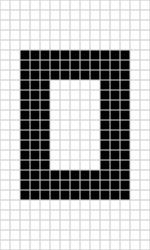
\includegraphics[height=1.5in]{zero.jpg}% 
}
\subcaptionbox{The three vector types in the `zero' matrix.}[0.4\linewidth]{%
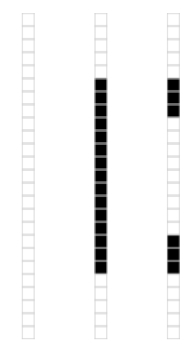
\includegraphics[height=1.5in]{zero-vecs.jpg}% 
}
\end{center}
\end{figure}

If SVD is working like expected it should capture that feature of our input matrix, and we should be able to represent the entire image using just three singular values and their associated left- and right-singular vectors.

\begin{Rcode}
> zsvd <- svd(z)
> round(zsvd$d,2)
 [1] 14.72  5.22  3.31  0.00  0.00  0.00  0.00  0.00  0.00  0.00  0.00  0.00  0.00  0.00
[15]  0.00
> D <- diag(zsvd$d[1:3])
> D
         [,1]     [,2]     [,3]
[1,] 14.72425 0.000000 0.000000
[2,]  0.00000 5.216623 0.000000
[3,]  0.00000 0.000000 3.314094
> U <- zsvd$u[,1:3]
> V <- zsvd$v[,1:3]
> newZ <- U %*% D %*% t(V)
> all.equal(newZ, zmatx, check.attributes=F)
[1] TRUE

# and let's double check using the image() function
> image(1:15,1:25,t(newZ),col=c('black','white'),asp=1)
\end{Rcode}

Our original matrix required $25 \times 15$ ($= 375$) storage elements. Using the SVD we can represent the same data using only $15 \times 3 + 25 \times 3 + 3 = 123$ units of storage (corresponding to the truncated U, V, and D in the example above). Thus our SVD allows us to represent the same data with at less than $1/3$ the size of the original matrix. In this case, because all the singular values after the 3rd were zero this is a lossless data compression procedure. 

\subsubsection*{Noise filtering using SVD}

The file |noisy-zero.dat| is the same 'zero' image, but now sprinkled with Gaussian noise draw from a normal distribution ($N(0,0.1)$. As in the data compression case we can use SVD to approximate the input matrix with a lower-dimensional approximation. Here the SVD is `lossy' as our approximation throws away information.  In this case we hope to choose the approximating dimension such that the information we lose corresponds to the noise which is `polluting' our data. 

\begin{Rcode}
> nz <- as.matrix(read.delim('noisey-ones.dat',header=F))
> dim(nz)
[1] 25 15
# create a gray-scale representation of the matrix
> image(x,y,t(nz),asp=1,xlim=c(1,15),ylim=c(1,25),col=gray(seq(0,1,0.05)))
> round(nz.svd$d,2)
 [1] 13.63  4.87  3.07  0.40  0.36  0.31  0.27  0.26  0.21  0.19  0.13  0.11  0.09  0.06
[15]  0.04
# as before the first three singular values dominate
> nD <- diag(nz.svd$d[1:3])
> nU <- nz.svd$u[,1:3]
> nV <- nz.svd$v[,1:3]
> approx.nz <- nU %*% D %*% t(nV)    

# now plot the original and approximating matrix side-by-side
> par(mfrow=c(1,2))
> image(x,y,t(nz),asp=1,xlim=c(1,15),ylim=c(1,25),col=gray(seq(0,1,0.05)))
> image(x,y,t(approx.nz),asp=1,xlim=c(1,15),ylim=c(1,25),col=gray(seq(0,1,0.05)))
\end{Rcode}

As you can see from the images you created the approximation based on the approximation based on the SVD manages to capture the major features of the matrix and filters out much of (but not all) the noise.

\subsection*{Image Approximation Using SVD in Python}

The Python Imaging Library (PIL) is a package of routines for manipulating image data in Python. If you're using the Enthought build of Python this was included in your installation. If building packages from scratch you can find the PIL at \href{http://www.pythonware.com/products/pil/}{http://www.pythonware.com/products/pil/} or pre-built binaries for OS X can be found at \href{http://www.pythonmac.org/packages/}{http://www.pythonmac.org/packages/}. Documentation on PIL is available \href{http://www.pythonware.com/library/pil/handbook/index.htm}{here}.

The PIL package provide a more general set of image manipulation features than does R.  In the exercises below we will use the PIL package in combination with |numpy| apply SVD to a more complicated image.

Download the module of helper functions \texttt{imagehelper.py} from the course wiki and place it somewhere in your \texttt{PYTHONPATH}. Also, download the JPEG image \texttt{chesterbw.jpg} and place it in a convenient directory such as |c:/temp| or |~/temp|. {\color{red} \bfseries I very strongly recommend you use IPython with the --pylab option to run the following code.}

\begin{Pcode}
>>> import numpy as np, numpy.linalg as la
>>> from matplotlib import pyplot
>>> import Image # this is the main module in the PIL package
>>> import imagehelper

>>>  # Let's load and examine our image
>>> cd ~/temp # change to wherever you save the image
>>> im = Image.open("chesterbw.jpg")
>>> im.size
(605, 556) # the image is 605 pixels x 556 pixels
>>> im.show() # assumes you have a default image viewer configured in your OS
 
>>> # matplotlib.pyplot also has an imshow function
>>> pyplot.imshow(im,origin='lower') # (0,0) is in lower left of image
<matplotlib.image.AxesImage object at 0x7aa6d90>
>>> pyplot.imshow(im,origin='lower',cmap='gray') # change the colormap to grayscale
<matplotlib.image.AxesImage object at 0x22e87c10>
>>>
>>>   # convert the image to an array
>>> imgarray = np.asarray(im)
>>> imgarray.shape
(556, 605)
>>> fimage = imgarray.astype(np.float32) # svd requires floating points

>>>   # Create a low dimensional approximation to our image
>>> U,S,Vt = la.svd(fimage)
>>> U15 = U[:,:15]
>>> S15 = np.eye(15) * S[:15] # eye() creates an identity matrix
>>> Vt15 = Vt[:15,:]
>>> approx15 = np.dot(U15, np.dot(S15, Vt15)) # 15 dim. approx. of original image
>>> approxim = imagehelper.array2image(approx15.astype(np.uint8))
>>> approxim.show()

>>>    # Use pyplot.matshow to view a image representation of a matrix directly
>>> pyplot.matshow(fimage, cmap='gray')
>>> pyplot.matshow(approx15, cmap='gray')

>>>    # lets calculate the difference between the two images and plot that
>>> imgdiff = fimage - approx15
>>> pyplot.matshow(imgdiff, cmap='gray')

>>>    # showing off some other features of matplotlib
>>> pyplot.imshow(fimage,cmap='gray_r') # reversed gray scale
>>> fig = pyplot.figure()
>>> fig.add_subplot(1,2,1)
>>> pyplot.imshow(fimage, cmap='gray')
>>> fig.add_subplot(1,2,2)
>>> pyplot.imshow(approx15, cmap='gray')

\end{Pcode}

Above we created a rank 15 approximation to the rank 556 original image matrix. This approximation is crude (as judged by the visual quality of the approximating image) but it does represent a very large savings in space. Our original image required the storage of $605 \times 556 = 336380$ integer values. Our approximation requires the storage of only $15 \times 556 + 15 \times 605 + 15 = 17430$ integers. This is a saving of roughly 95\%. Of course, as with any lossy compression algorithm, you need to decide what is the appropriate tradeoff between compression and data loss for your given application.

The Python Image Library has lots of useful functions for manipulating image data. You might spend some time checking out the documenation (see the PIL homepage given above). For more info on the Matplotlib built in color maps see: \href{http://matplotlib.sourceforge.net/examples/pylab_examples/show_colormaps.html}{Matplotlib colormaps}.



\begin{assignment}
Write a function (|svd_img()|) in Python that automates the creation of a lower dimensional approximation of a grayscale image using SVD.  Test your function on various images using a variety of approximating dimensions (e.g. 5,10, 25, 50, 100, 250 on the \texttt{chesterbw.jpg} image).  Your function should take as input a floating point array representing the original image and an integer specifying the approximating dimension (i.e. function will be called as |svd_img(imgarray,dim)|). Your function should return two objects: 1) an array representing the approximated image; and 2) an array representing the difference between the original and approximating images.

In addition to your code consider the following questions:

\begin{itemize}
\item When analyzing \texttt{chesterbw.jpg}, at some approximating dimensions you'll notice interesting artifacts. How do these relate to the original image? 

\item What is the lowest approximating dimension where you would you consider the image to be recognizable as a dog?
 
\item At what approximating dimension would you judge the  image to be ``close enough"  to the original by the casual observer? What is the storage saving of this approximation relative to the original image?

\item How does the difference array (original - approximating) change as the approximating dimension changes? Is there a particular type of image information that seems most prominent in the difference array?
\end{itemize}

\textbf{Extra credit}: write a function (|svd_img_plot()|)that creates a single figure in matplotlib that with three subfigures that compare the original, approximating, and difference arrays. 

\end{assignment}






% 
% \section*{Correspondence Analysis in R}
% 
% There is no built-in function in R for doing correspondence analysis. However, a simple correspondence analysis function is found in the \texttt{MASS} package. Here we recreate the correspondence analysis for a contigency table that relates hair color (columns) to eye color (rows) in sample taken in a town in Scotland.
% 
% \begin{Rcode}
% > ?corresp
% > library(MASS)
% > caith
%        fair red medium dark black
% blue    326  38    241  110     3
% light   688 116    584  188     4
% medium  343  84    909  412    26
% dark     98  48    403  681    85
% > corresp(caith)
% First canonical correlation(s): 0.4463684 
% 
%  Row scores:
%        blue       light      medium        dark 
% -0.89679252 -0.98731818  0.07530627  1.57434710 
% 
%  Column scores:
%        fair         red      medium        dark       black 
% -1.21871379 -0.52257500 -0.09414671  1.31888486  2.45176017 
% > biplot(corresp(caith,nf=2))
% \end{Rcode}
% 
% For a different implementation of correspondence analysis and related methods as well as other functions related to ecological data analysis you should check out the \texttt{ade4} and \texttt{vegan} (for vegetation analysis) packages. See the \texttt{ade4} webpage at \href{http://pbil.univ-lyon1.fr/ADE-4/}{http://pbil.univ-lyon1.fr/ADE-4/}. See the \texttt{vegan} webpage at \href{http://cc.oulu.fi/~jarioksa/softhelp/vegan.html}{http://cc.oulu.fi/~jarioksa/softhelp/vegan.html}.

\end{document}
